\scanpage{19}
\mspage{18}
\mspage{IV-953}

En effet, $Y$ étant compact \deleted{\unsure{et}} et noethérien, toute partie de $Y$ est compacte, donc fermée, ce qui implique que $Y$ est discret, donc fini puisqu'il est compact.

\uline{Corollaire} (18.6.10).-- \uline{Soit} $A$ \uline{un anneau local noethérien. Pour que} ${}^h A$ \uline{possède une des propriétés suivantes} :

a) \uline{être un anneau de Cohen-Macaulay} ;

b) \uline{vérifier la propriété} $(S_n)$ ;

c) \uline{être régulier} ;

d) \uline{vérifier la propriété} $(R_n)$ ;

\margin{\figure{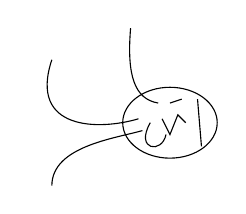
\begin{tikzpicture}[x=1cm,y=1cm]\draw (1,2) .. controls (.95,1.4) and (1.05,1.1) .. (1.35,1.05);\draw (0,1.6) .. controls (-.3,.7) and (.6,.7) .. (1.1,.85);\draw (0,0) .. controls (0,.5) and (.8,.6) .. (1.15,.7);\draw (1.25,.8) .. controls (1.05,.45) and (1.4,.4) .. (1.45,.65);\draw (1.4,.85)--(1.5,.65)--(1.6,.9)--(1.7,.8);\draw (1.5,1.05)--(1.65,1.1);\draw (1.85,1.1)--(1.9,.5);\draw (1.5,.8) ellipse (.6 and .45);\end{tikzpicture}}}

\uline{il faut et il suffit que} $A$ \uline{possède cette même propriété}.

Cela résulte aussitôt de ce que les fibres du morphisme $\operatorname{Spec}({}^h A)\to\operatorname{Spec}(A)$ sont géométriquement régulières (18.6.9) et de (6.4.1), (6.5.1) et (6.5.3).

\uline{Corollaire} (18.6.11).-- \uline{Soit} $A$ \uline{un anneau semi-local noethérien. Pour qu'un idéal premier} $\underline p$ \uline{de} ${}^h A$ \uline{appartienne à} $\operatorname{Ass}({}^h A)$, \uline{il faut et il suffit que} $\underline p\cap A$ \uline{appartienne à} $\operatorname{Ass}(A)$.

Compte tenu de la description des fibres du morphisme $\operatorname{Spec}({}^h A)\to\operatorname{Spec}(A)$, cela résulte aussitôt de (3.3.1).

\uline{Proposition} (18.6.1\deleted{\unsure{1}}\inserted{2}).-- \uline{Soi\deleted{\unsure{en}}t} $A$ \uline{un anneau local ; les propriétés suivantes sont équivalentes} :

a) $A$ \uline{est unibranche} (resp. \uline{réduit et unibranche}).
\margin{\figure{\begin{tikzpicture}[x=1cm,y=1cm]\draw (0,0) .. controls (0,.5) and (.25,.8) .. (.6,.85);\draw (.7,.9)--(.75,.82);\draw (.9,.9)--(.94,.86);\draw (1.1,1.05)--(1.18,.6);\end{tikzpicture}}}

b) \uline{Pour toute} $A$-\uline{algèbre locale strictement essentiellement étale} $A'$, \deleted{\unsure{Spec}} $\operatorname{Spec}(A')$ \uline{est irréductible} (resp. \uline{intègre}).

c) $\operatorname{Spec}({}^h A)$ \uline{est irréductible} (resp. \uline{intègre}).

Notons d'abord que ${}^h(A_{\mathrm{red}})=({}^h A)_{\mathrm{red}}$, car \deleted{\illegible{13}} ${}^h(A_{\mathrm{red}})=({}^h A)\otimes_A A_{\mathrm{red}}$ (18.6.8), et comme ${}^h(A_{\mathrm{red}})$ est réduit (18.6.9), il est égal à $({}^h A)_{\mathrm{red}}$. Ceci permet, dans la démonstration, de considérer seulement le cas où $A$ est \uline{réduit}, donc aussi $A'$ (17.5.7) et ${}^h A$ (18.6.9).

\deleted{\unsure{Il est clair que}} Avec les notations de (18.6.4), la condition b) signifie que tous les $A_\alpha$ sont intègres ; \deleted{comme les homomorphismes $\unsure{A_\alpha\to A_\beta|A_\alpha\to{}^h A}$ sont \unsure{injectifs}} on en conclut que ${}^h A=\varinjlim A_\alpha$ est intègre (5.13.3), donc b) entraîne c).

